\section{Introduction} 

\begin{figure}[t] \begin{center}
    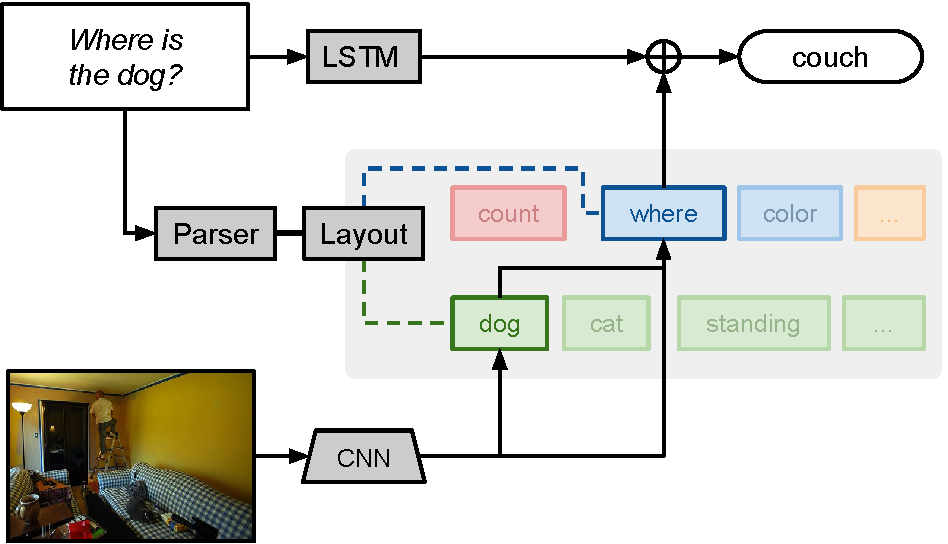
\includegraphics[width=\linewidth]{fig/teaser} \end{center} \caption{Our
    approach answers questions about images, it automatically instantiates
    different modules of neural networks depending on the question. An
    additional LSTM provides sentence context and learns common sense / dataset
  bias.} \label{fig:teaser}
\end{figure}

This paper describes a framework for answering natural language questions with
collections of jointly-trained neural ``modules'', using linguistic structure to
dynamically assemble these modules into deep networks. Our initial focus is on
visual question answering, a task with significant applications to human-robot
interaction, search, and accessibility. Visual QA is the subject of a great deal
of current research attention 
\cite{antol15iccv,gao2015you,ma15arxiv,malinowski15iccv,ren2015image,yu15arxiv}, 
requiring sophisticated understanding of both visual scenes and natural
language.

Specifically, given an image and an associated question (e.g.\ \emph{where is
the dog?}), we wish to predict a corresponding answer (e.g.\ \emph{on the couch},
or perhaps just \emph{couch}). Recent successful represent questions as
bag-of-words \cite{} or read in the question using a single neural network
\cite{malinowski15iccv}\cite{} and train a classifier on the full question
representation and the full-image representation. In contrast to these
monolithic approaches, another line of work for textual QA \cite{Liang13DCS} and
image QA \cite{malinowski14nips} uses semantic parsers to decompose questions
into logical expressions. These logical expressions are evaluated against a
logical representation of the world, which may be provided directly or extracted
from an image \cite{Krish2013Grounded}.

In this paper we draw from both lines of research, presenting a technique for
integrating the representational power of neural networks with the flexible
compositional structure afforded by symbolic approaches to semantics.  Rather
than relying on a monolithic network structure to answer all questions, our
approach assembles a network on the fly from a collection of specialized,
jointly-learned modules (\autoref{fig:teaser}). In particular, we first analyze
the question with an off-the-shelf semantic parser, and use this analysis to
determine the basic computational units (detection, classification, etc.) needed
to answer the question, as well as the relationships between them. In
\autoref{fig:teaser}, we first produce a dog detector, which sends its output to
a location classifier. Depending on the underlying structure, these messages
passed between modules may be raw image features, attentions, or classification
decisions; each module is determined by its input and output types.
Different kinds of modules are marked with different
colors in \Figref{fig:teaser}: for example the \mod{attend[$dog$]} module
(green) produces a spatial heatmap while the \mod{classify[$where$]} (blue)
produces a classification output, given an attention heatmap and the image
content. Importantly, all modules of a NMN are independent, which allows the
computation to be different for each problem instance, and possibly unobserved
during training. 
%So that we can answer novel question at test time, such as
%\emph{Where is the banana?}, even we only saw \emph{count} or
%\emph{color} question about \emph{bananas} during training.  
In addition to the NMN our final answer also incorporates the image scene
knowledge (using a full frame CNN) and uses an  recurrent network (LSTM) to read
the question, which has been shown to be important to model common sense
knowledge and dataset biases \cite{malinowski15iccv}.

%Where previous work has
%treated both the image and the question as inputs to a monolithic
%classification model, we instead take the perspective that a question is a
%noisy specification of a hidden computation that must be performed on the image
%to produce an answer. Crucially, this computation may be different for each
%problem instance, and is never observed observed during training.

%Our approach bears a superficial resemblance to a classical semantic parser.
%However, instead of mapping from questions to logical forms, our model maps
%from questions to neural network structures. These networks are assembled on
%the fly (possibly into novel topologies) from a collection of jointly-learned
%neural ``modules''. Finally, they are evaluated against the input image to
%produce an answer.




%This paper presents a technique for following natural language instructions
%(and performing other dynamically-specified tasks) by assembling deep neural
%networks on the fly from an inventory of pre-trained components.

We evaluate our approach on three visual question answering tasks. On the
recently-released CocoQA \cite{yu15arxiv} and  VQA \cite{antol15iccv} datasets,
we achieve results comparable to [better than] existing approaches, and show
that our approach specifically outperforms previous work on questions with
compositional structure (\eg requiring that an object be located and one of its
attributes described). Using our model on questions where compositional
structure plays a central role, and falling back to previous approaches
elsewhere, we achieve new state-of-the-art results on both tasks. It turns out,
however, that most of the questions in both datasets are quite simple, with
little composition. To test our approach's ability to handle highly structured
questions, we introduce a new dataset of synthetic images paired with complex
questions involving spatial relations, set-theoretic reasoning, and shape and
attribute recognition. On this dataset we outperform the previous state of the
art by XXX.

While all the applications considered in this paper involve visual question
answering, the general architecture is potentially of broader usefulness, and
might be more generally applied to referring expression resolution (XXX),
question answering about natural language texts (XXX), or XXX.

%We evaluate our approach on two visual question answering tasks. First we
%present a new synthetic image dataset paired with a complex set of queries
%(involving spatial relations, logical operators, and shape and attribute
%recognition). Next, we consider a hard subset of the Microsoft VQA corpus of
%questions about natural images. In each case, an NMN-based approach outperforms
%state-of-the-art models with more conventional recurrent architectures. We
%observe in particular that NMNs are able to make considerably better use of
%small training sets.

To summarize our contributions: We first propose neural module networks, a
general architecture for discretely composing heterogeneous, jointly-trained
neural modules into deep networks. Next, for the visual QA task specifically, we
show how to construct NMNs based on the output of a semantic parser, and use
these to successfully complete established visual question answering tasks.
Finally, we introduce a new dataset of challenging, highly compositional
questions about abstract shapes, and show that our approach outperforms previous
models by as much as XXX. We will release this dataset, as well as code for all
systems described in this paper, at $<anonymous>$.
